\section{Budget-Constrained Pacing}
\label{sec:pacing_results}
\label{sec:exp3_results}

This section studies constraint-driven bid suppression, where budget-constrained pacing agents suppress bids to ration a finite budget across auctions, in contrast to the learning-driven suppression observed in earlier experiments. We study this mechanism using multiplicative dual pacing \citep{Balseiro2019Learning} in Experiment~3a and proportional-integral control in Experiment~3b.

\subsection{Design}
\label{sec:shared_env_pacing}
\label{sec:exp3_appendix}

Experiments~3a and~3b share a common auction environment. Each of $n \in \{2, 4\}$ advertisers participates in a sequence of $D = 100$ episodes, each comprising $T = 1{,}000$ single-item auctions. Between episodes, budgets regenerate to their initial level while control variables persist (warm-starting).

Valuations follow a log-normal model with bidder-specific asymmetry. Each bidder $i$ draws a mean $\mu_i \sim \mathrm{Uniform}(0.5, 1.5)$ once per seed. In each round $t$, the valuation $v_{it} \sim \mathrm{LogNormal}(\mu_i, \sigma)$ with $\sigma \in \{0.1, 0.5\}$. The budget per bidder per episode is $B_i = m \cdot \mathbb{E}[v_{it}] \cdot T$, where $\mathbb{E}[v_{it}] = \exp(\mu_i + \sigma^2/2)$ and $m \in \{0.25, 1.0\}$ is the budget multiplier. The auction may impose a reserve price $r \in \{0.0, 0.3\}$. Bids below $r$ are excluded, and in second-price auctions the payment is the maximum of the second-highest bid and $r$.

\label{sec:exp3a_design}
\label{sec:exp3a_appendix}

All bidders use a multiplicative dual pacing algorithm. In each round the agent computes a bid as a function of its current dual variable $\mu_t$:
\begin{align}
  b_{it} &= \min\!\Big(\frac{v_{it}}{\mu_t},\; B_i - S_{it}\Big) & &\text{(value-maximizer),} \label{eq:bid_vmax} \\
  b_{it} &= \min\!\Big(\frac{v_{it}}{1 + \mu_t},\; B_i - S_{it}\Big) & &\text{(utility-maximizer),} \label{eq:bid_umax}
\end{align}
where $S_{it}$ is the cumulative spend at round $t$. The dual update follows
\begin{equation}
  \mu_{t+1} = \mathrm{clip}\!\Big(\mu_t \cdot \exp\!\big(\alpha_p\,(p_t - \rho)\big),\; 10^{-4},\; 100\Big),
  \label{eq:dual_update_exp3a}
\end{equation}
with step size $\alpha_p = 1/\sqrt{T}$ and target spend rate $\rho = B_i / T$.

\subsubsection{Factorial Design}

The experiment uses a $2^6 = 64$ cell full factorial with six factors (Table~\ref{tab:exp3a_params}). Each cell is replicated across independent seeds, yielding \ExpThreeANobs{} total runs. This design estimates all main effects and two-way interactions without aliasing.

\begin{table}[H]
\centering
\caption{Parameter settings for Experiment~3a (Budget-Constrained Pacing).}
\label{tab:exp3a_params}
\begin{tabular}{l l l}
\toprule
\textbf{Factor} & \textbf{Low ($-1$)} & \textbf{High ($+1$)}\\
\midrule
Auction format & Second-price & First-price \\
Bidder objective & Value-maximizer & Utility-maximizer \\
Number of bidders ($n$) & 2 & 4 \\
Budget multiplier ($m$) & 0.25 (tight) & 1.0 (loose) \\
Reserve price ($r$) & 0.0 & 0.3 \\
Value dispersion ($\sigma$) & 0.1 (low) & 0.5 (high) \\
\midrule
\multicolumn{3}{l}{\textbf{Fixed parameters}} \\
\midrule
Episodes ($D$) & \multicolumn{2}{l}{100} \\
Rounds per episode ($T$) & \multicolumn{2}{l}{1{,}000} \\
Log-normal $\mu$ range & \multicolumn{2}{l}{$[0.5, 1.5]$} \\
Initial $\mu_0$ & \multicolumn{2}{l}{1.0} \\
Burn-in episodes & \multicolumn{2}{l}{10} \\
\bottomrule
\end{tabular}
\end{table}

\label{sec:exp3b_design}
\label{sec:exp3b_appendix}

Experiment~3b replaces the multiplicative dual pacing with a proportional-integral (PI) controller. The PI controller computes a spending error $e_t = (t/T)\,B^i - S_{it}$ at each round, where $S_{it}$ is cumulative spend, and updates the bid multiplier:
\begin{align}
  e_t^i &= \tfrac{t}{T}\,B^i - {\textstyle\sum_{\tau \le t}} c_\tau^i, \label{eq:pid_error_exp3b}\\
  \lambda_{t+1}^i &= \operatorname{clip}\!\bigl(\lambda_t^i + K_P\,e_t^i + K_I\!\textstyle\sum_{\tau} e_\tau^i,\; 0.01,\; 1.5\bigr), \label{eq:pid_update_exp3b}
\end{align}
with $K_P = 0.30 \times a$ and $K_I = 0.05 \times a$, where $a$ is the aggressiveness parameter. The agent bids $b_t = \min(\lambda_t \cdot v_t,\; B^i - S_t^i)$.

The competitive benchmark is $\lambda = 1$ (full-value bidding) for both auction formats.

\subsubsection{Factorial Design}

The experiment uses a $2^6 = 64$ cell full factorial with six factors (Table~\ref{tab:exp3b_params}). The aggressiveness factor replaces the bidder objective factor from Experiment~3a, testing how controller responsiveness affects bidding outcomes. Each cell is replicated across 8 independent seeds for 512 total runs.

\begin{table}[H]
\centering
\caption{Parameter settings for Experiment~3b (PI Controller Pacing).}
\label{tab:exp3b_params}
\begin{tabular}{l l l}
\toprule
\textbf{Factor} & \textbf{Low ($-1$)} & \textbf{High ($+1$)}\\
\midrule
Auction format & Second-price & First-price \\
Aggressiveness $a$ & 0.3 (conservative) & 3.0 (aggressive) \\
Number of bidders ($n$) & 2 & 4 \\
Budget multiplier ($m$) & 0.25 (tight) & 1.0 (loose) \\
Reserve price ($r$) & 0.0 & 0.3 \\
Value dispersion ($\sigma$) & 0.1 (low) & 0.5 (high) \\
\midrule
\multicolumn{3}{l}{\textbf{Fixed parameters}} \\
\midrule
Episodes ($D$) & \multicolumn{2}{l}{100} \\
Rounds per episode ($T$) & \multicolumn{2}{l}{1{,}000} \\
Log-normal $\mu$ range & \multicolumn{2}{l}{$[0.5, 1.5]$} \\
Initial $\lambda_0$ & \multicolumn{2}{l}{1.0} \\
Burn-in episodes & \multicolumn{2}{l}{10} \\
$K_P$ & \multicolumn{2}{l}{$0.30 \times a$} \\
$K_I$ & \multicolumn{2}{l}{$0.05 \times a$} \\
\bottomrule
\end{tabular}
\end{table}

The aggressiveness factor scales the PI controller gains by a factor of $10\times$ (from $a = 0.3$ to $a = 3.0$). The proportional gain $K_P$ ranges from $0.09$ to $0.90$ and the integral gain $K_I$ from $0.015$ to $0.15$. Higher aggressiveness produces faster budget consumption and more reactive pacing, while lower aggressiveness yields conservative, slow-adjusting behaviour. The $10\times$ ratio ensures meaningful separation in controller dynamics without pushing either level into degeneracy (budget exhaustion in the first few rounds or near-zero spending).\footnote{In Experiment~3a, the bidder objective factor contrasts value-maximisation ($b = v/\mu$) with utility-maximisation ($b = v/(1+\mu)$), two structurally different bidding rules drawn from the price of anarchy literature. The asymmetry is definitional, not parametric.}


The following metrics are computed per run by averaging over the 90 post-burn-in episodes ($d \geq 10$):

\begin{table}[H]
\centering
\small
\caption{Experiment~3a response variables.}
\label{tab:exp3a_responses}
\begin{tabular}{ll}
\toprule
\textbf{Metric} & \textbf{Definition} \\
\midrule
Platform revenue       & Total payments per episode \\
Liquid welfare         & $\sum_i \min(B_i,\; \text{total value won by } i)$ per episode \\
Effective PoA          & LP offline optimum / liquid welfare \\
Budget utilisation     & Mean spend/budget across bidders \\
Bid-to-value ratio     & Mean $b/v$ across all bids \\
Allocative efficiency  & Fraction of rounds won by highest-value bidder \\
Dual variable CV       & CV of dual in last 200 rounds \\
No-sale rate           & Fraction of rounds with no valid bids \\
Winner entropy         & Shannon entropy of winner distribution \\
Warm-start benefit     & Revenue improvement episode~2 vs.~episode~1 \\
Inter-episode volatility & CV of revenue across post-burn-in episodes \\
Bid suppression ratio  & Observed btv / competitive btv \\
Cross-episode drift    & Slope of btv across episodes \\
\bottomrule
\end{tabular}
\end{table}

The effective PoA metric compares realised liquid welfare against offline optima computed with full hindsight. Section~\ref{sec:welfare} establishes the LP relaxation as an upper bound on achievable liquid welfare. Experiment~3b uses the same response variables (Table~\ref{tab:exp3a_responses}), with the dual variable CV computed from $\lambda$ history rather than $\mu$ history and the bid suppression ratio using a competitive benchmark of $\lambda = 1.0$ (full-value bidding). Analysis applies the same factorial ANOVA engine used in Experiments~1a through~2b to the run-level data, treating each seed as an independent replicate within its factorial cell.

\subsection{Dual Pacing Results (Experiment~3a)}
\label{sec:exp3a_results}

The design and factor levels are given in Table~\ref{tab:exp3a_params} (\ExpThreeANobs{} runs total).

\begin{figure}[H]
  \centering
  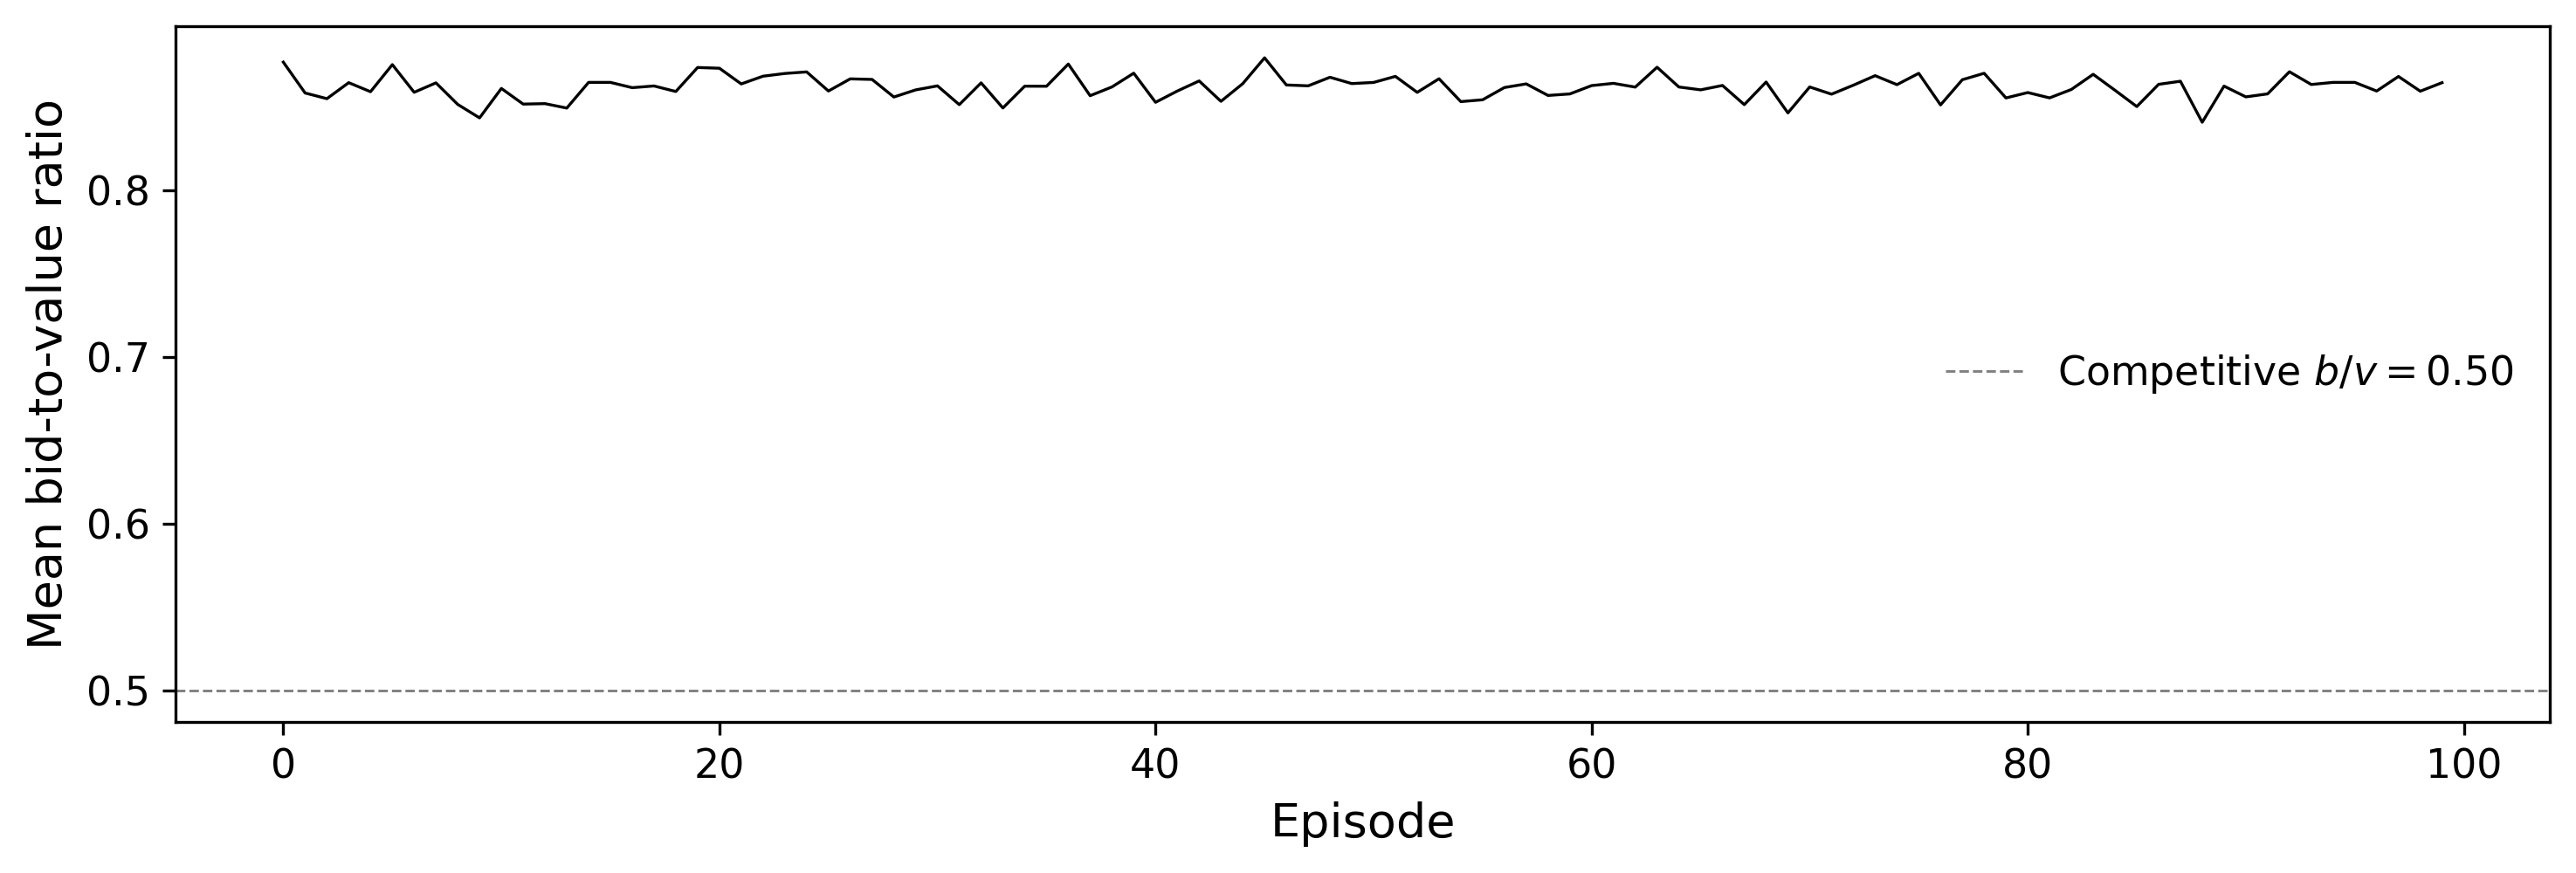
\includegraphics[width=\textwidth]{figures/e3a_trace}
  \caption{Representative learning trajectory for a single trial of Experiment~3a (first-price auction, value-maximizer objective, 2~bidders, 100 episodes $\times$ 1{,}000 rounds). Mean bid-to-value ratio per episode with the competitive benchmark (unconstrained Nash equilibrium $b/v = 0.5$).}
  \label{fig:e3a_trace}
\end{figure}

\subsubsection{Efficiency and Welfare}

Tables~\ref{tab:exp3a_ranked_rev} and~\ref{tab:exp3a_ranked_poa} report the ranked significant effects for platform revenue and effective Price of Anarchy, respectively. Response variable definitions appear in Table~\ref{tab:exp3a_responses}.

\begin{table}[H]
\centering
\caption{Experiment 3a: Significant effects for average revenue ($p < 0.05$), ranked by $|t|$.}
\label{tab:exp3a_ranked_rev}
\begin{tabular}{lrrl}
\toprule
\textbf{Effect} & \textbf{Coeff.} & \textbf{$|t|$} & \textbf{Direction} \\
\midrule
Budget multiplier & 2006.6019 & 39.44 & + \\
Bidder objective & -1428.0108 & 28.07 & $-$ \\
Bidder objective $\times$ Budget multiplier & -1387.4815 & 27.27 & $-$ \\
Number of bidders & 1158.2655 & 22.76 & + \\
Bidder objective $\times$ Number of bidders & -629.6958 & 12.38 & $-$ \\
Number of bidders $\times$ Budget multiplier & 448.9495 & 8.82 & + \\
Value dispersion ($\sigma$) & 356.7849 & 7.01 & + \\
Auction format & 184.0336 & 3.62 & + \\
Auction format $\times$ Bidder objective & 182.7252 & 3.59 & + \\
Auction format $\times$ Budget multiplier & 140.8645 & 2.77 & + \\
\bottomrule
\end{tabular}
\end{table}


\begin{figure}[H]
  \centering
  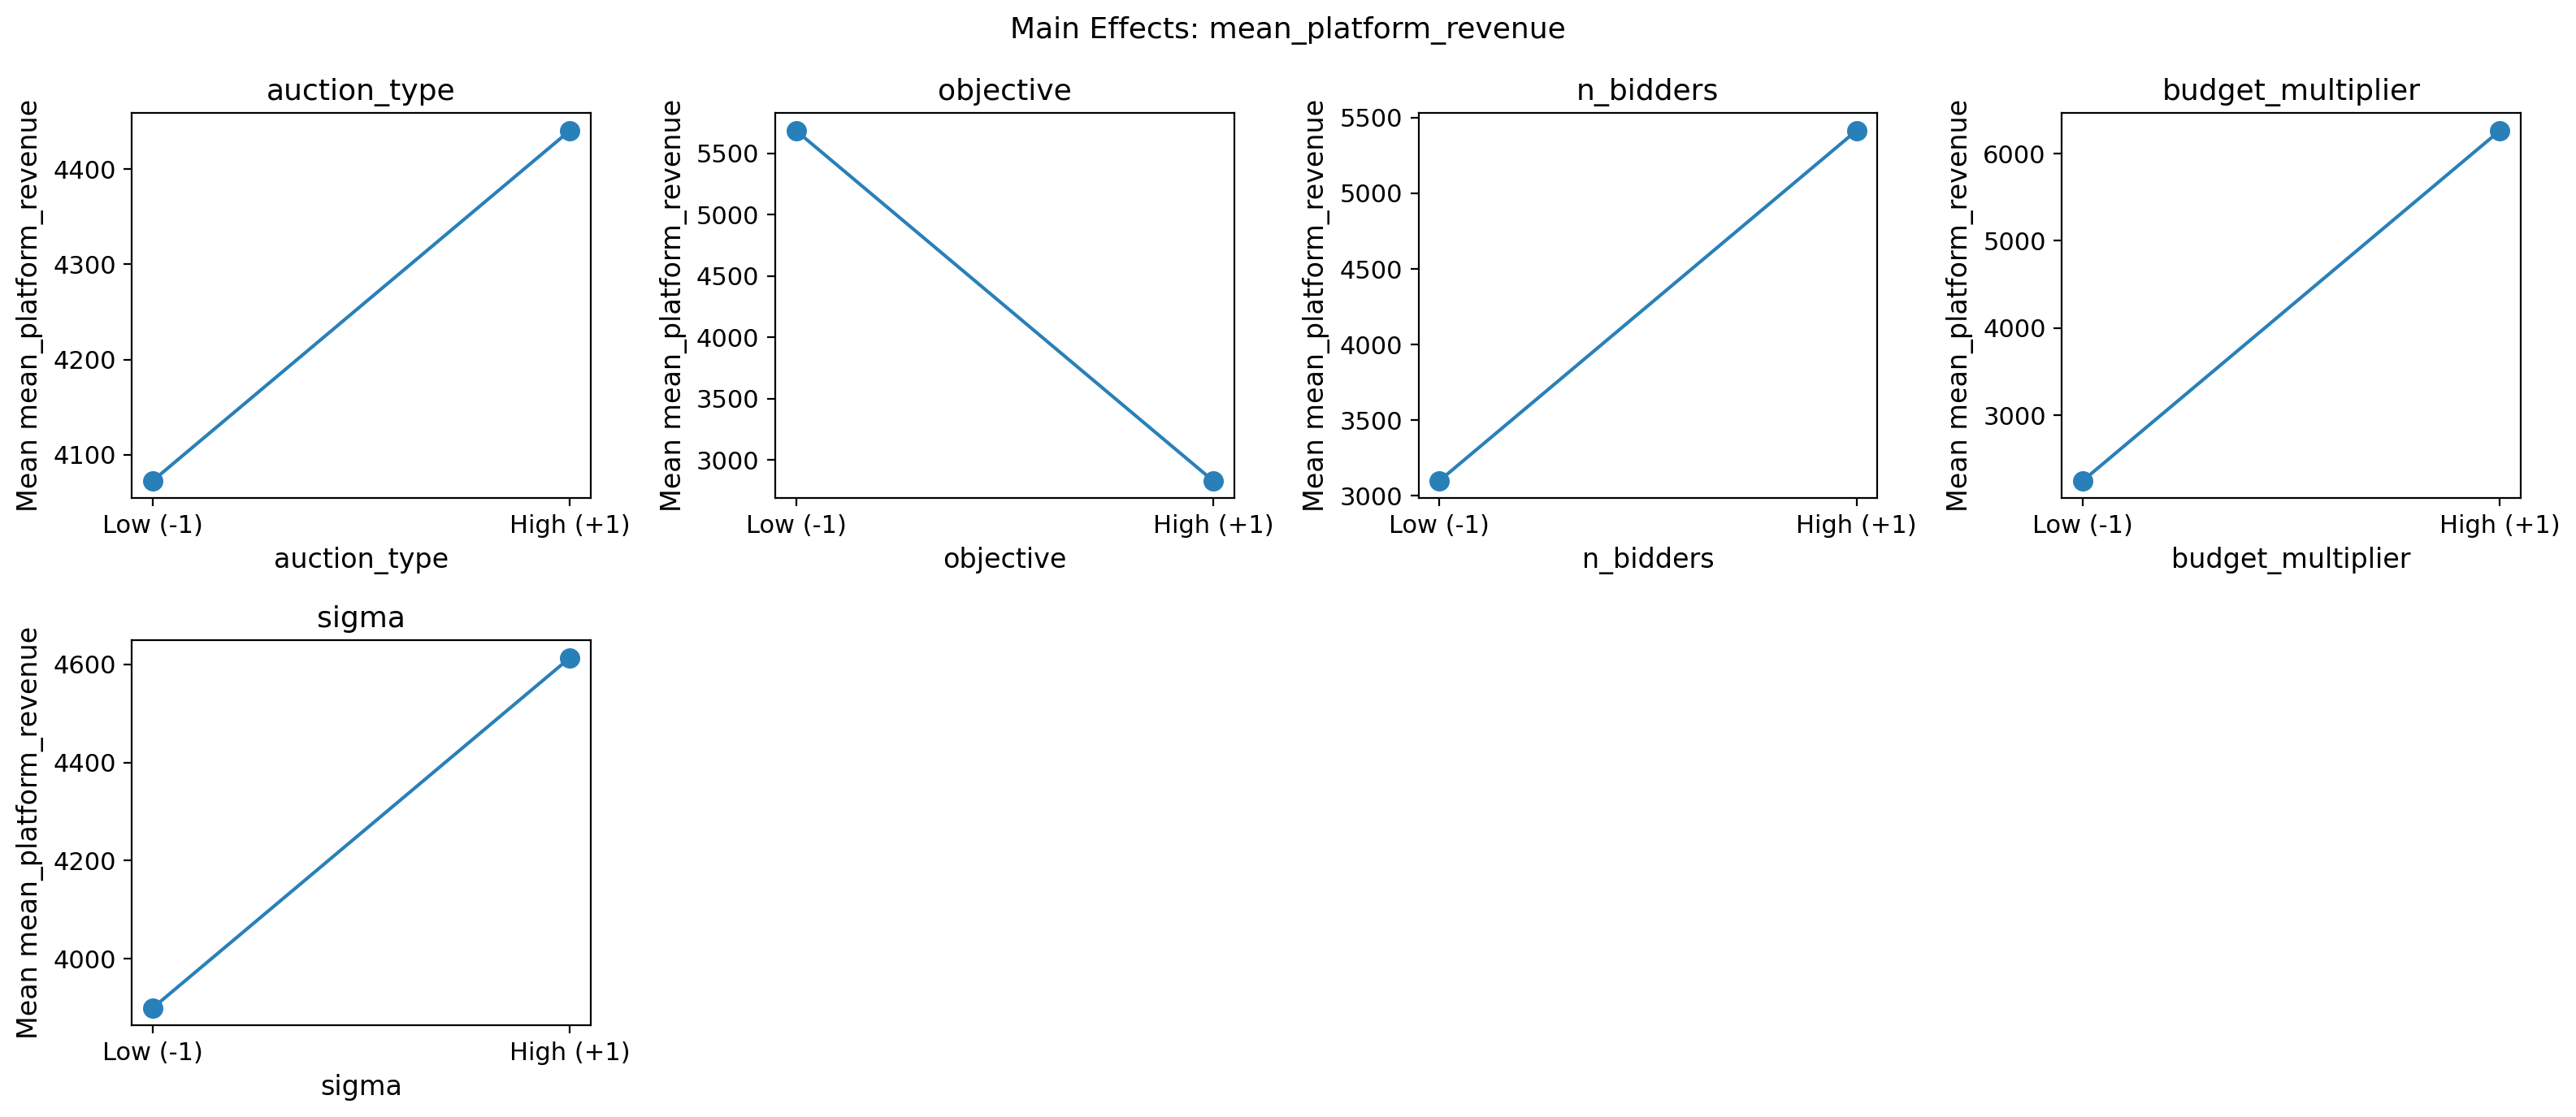
\includegraphics[width=0.7\textwidth]{figures/e3a_main_rev}
  \caption{Experiment~3a: Main effects plot for platform revenue across the three factors.}
  \label{fig:e3a_main_rev}
\end{figure}

\begin{table}[H]
\centering
\caption{Experiment 3a: Significant effects for effective Price of Anarchy ($p < 0.05$), ranked by $|t|$.}
\label{tab:exp3a_ranked_poa}
\begin{tabular}{lrrl}
\toprule
\textbf{Effect} & \textbf{Coeff.} & \textbf{$|t|$} & \textbf{Direction} \\
\midrule
Bidder objective $\times$ Budget multiplier & -0.0301 & 17.59 & $-$ \\
Bidder objective & -0.0205 & 12.01 & $-$ \\
Number of bidders & 0.0201 & 11.76 & + \\
Value dispersion ($\sigma$) & -0.0182 & 10.63 & $-$ \\
Budget multiplier & 0.0149 & 8.69 & + \\
Number of bidders $\times$ Value dispersion ($\sigma$) & -0.0142 & 8.28 & $-$ \\
Bidder objective $\times$ Number of bidders & -0.0042 & 2.48 & $-$ \\
Bidder objective $\times$ Value dispersion ($\sigma$) & 0.0039 & 2.29 & + \\
\bottomrule
\end{tabular}
\end{table}


\begin{figure}[H]
  \centering
  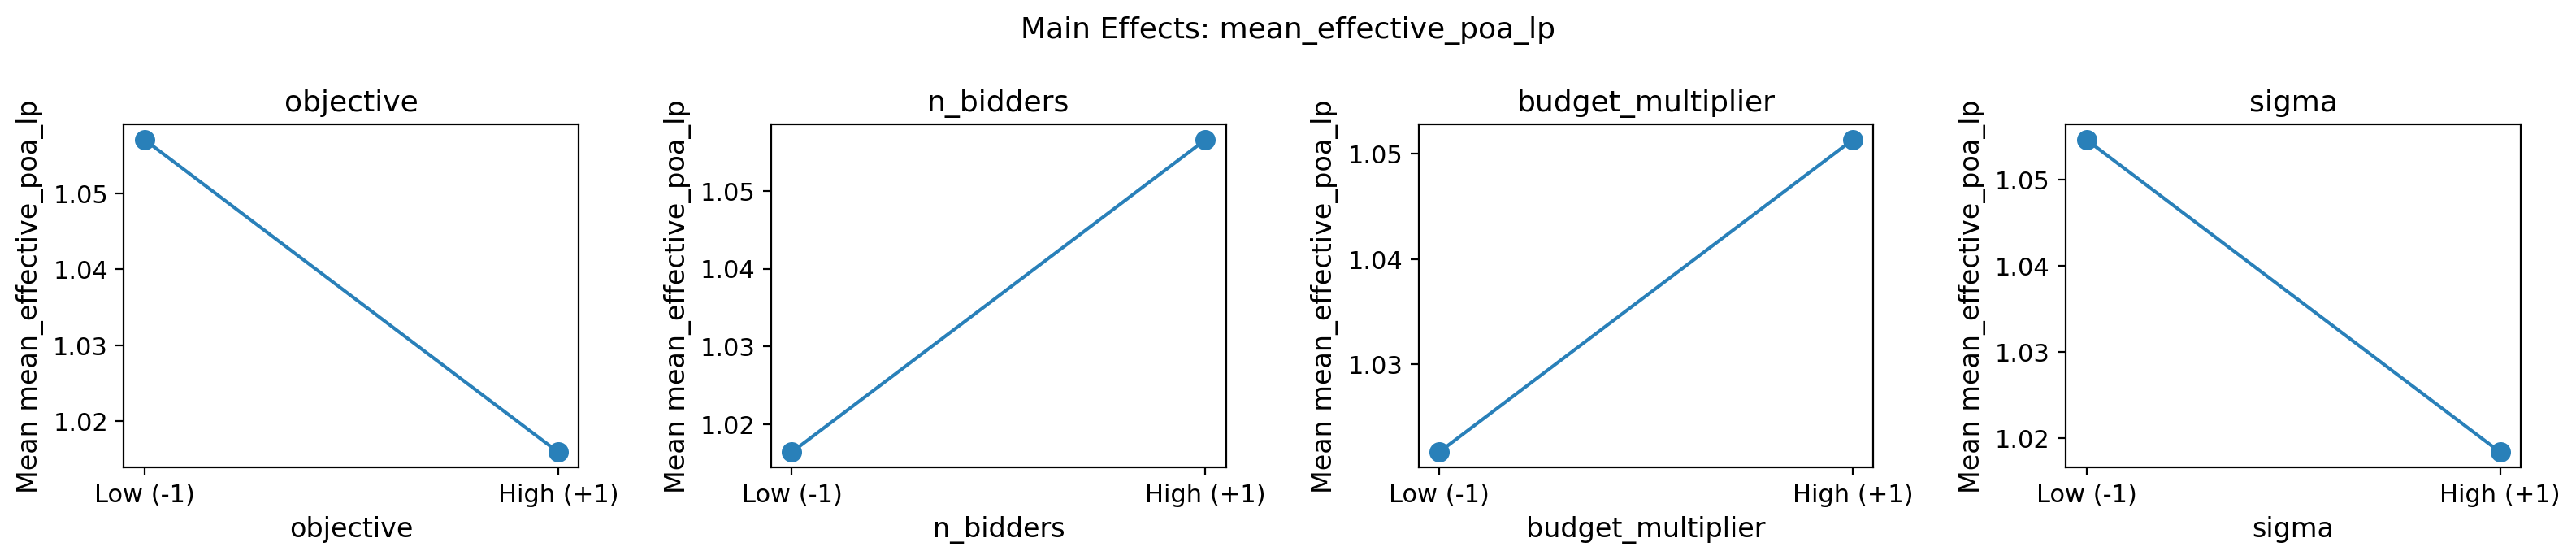
\includegraphics[width=0.7\textwidth]{figures/e3a_main_poa}
  \caption{Experiment~3a: Main effects plot for effective Price of Anarchy.}
  \label{fig:e3a_main_poa}
\end{figure}

All observed PoA values are well within the theoretical bound of~2 \citep{Aggarwal2019, Gaitonde2023}. The absence of a significant auction format effect on PoA contrasts with the revenue results. First-price bid suppression reduces payments to the auctioneer without proportionally distorting allocative outcomes. Allocative efficiency, the fraction of rounds in which the highest-value bidder wins, provides a complementary view. Under utility-maximizing objectives, agents achieve near-perfect efficiency. Under value-maximizing objectives with four bidders, efficiency drops substantially, with bid-to-value ratios exceeding 1.5.\footnote{Utility-maximizing efficiency ranges from \ExpThreeAUtilEffLow{} to \ExpThreeAUtilEffHigh{} across cells; value-maximizing four-bidder efficiency drops to \ExpThreeAValFourEffLow--\ExpThreeAValFourEffHigh, with bid-to-value ratios exceeding 1.5.} The objective$\times$n\_bidders interaction ($t = \ExpThreeAAllocEffObjxNbidT$, $p \ExpThreeAAllocEffObjxNbidPFmt$) captures this pattern, with the efficiency cost of value-maximizing objectives larger under four bidders than under two.

\subsubsection{Revenue and Budget Dynamics}

The budget multiplier dominates platform revenue ($|t| = \ExpThreeARevFactorTOne$), shifting revenue by \ExpThreeARevTopPctEffect\% of the grand mean. Tight budgets produce lower bids regardless of other design choices, while loose budgets produce higher bids and greater competitive intensity. The number of bidders ranks fourth ($|t| = \ExpThreeARevNbidAbsT$) and auction format fifth ($|t| = \ExpThreeARevAuctionT$). Table~\ref{tab:exp3a_ranked_rev} reports the full hierarchy. The interaction plot (Figure~\ref{fig:e3a_int_rev}) reveals how factor combinations jointly shape revenue outcomes. Market thickness interacts with auction format, with the revenue gap between formats widening as the number of bidders increases.

\begin{figure}[H]
  \centering
  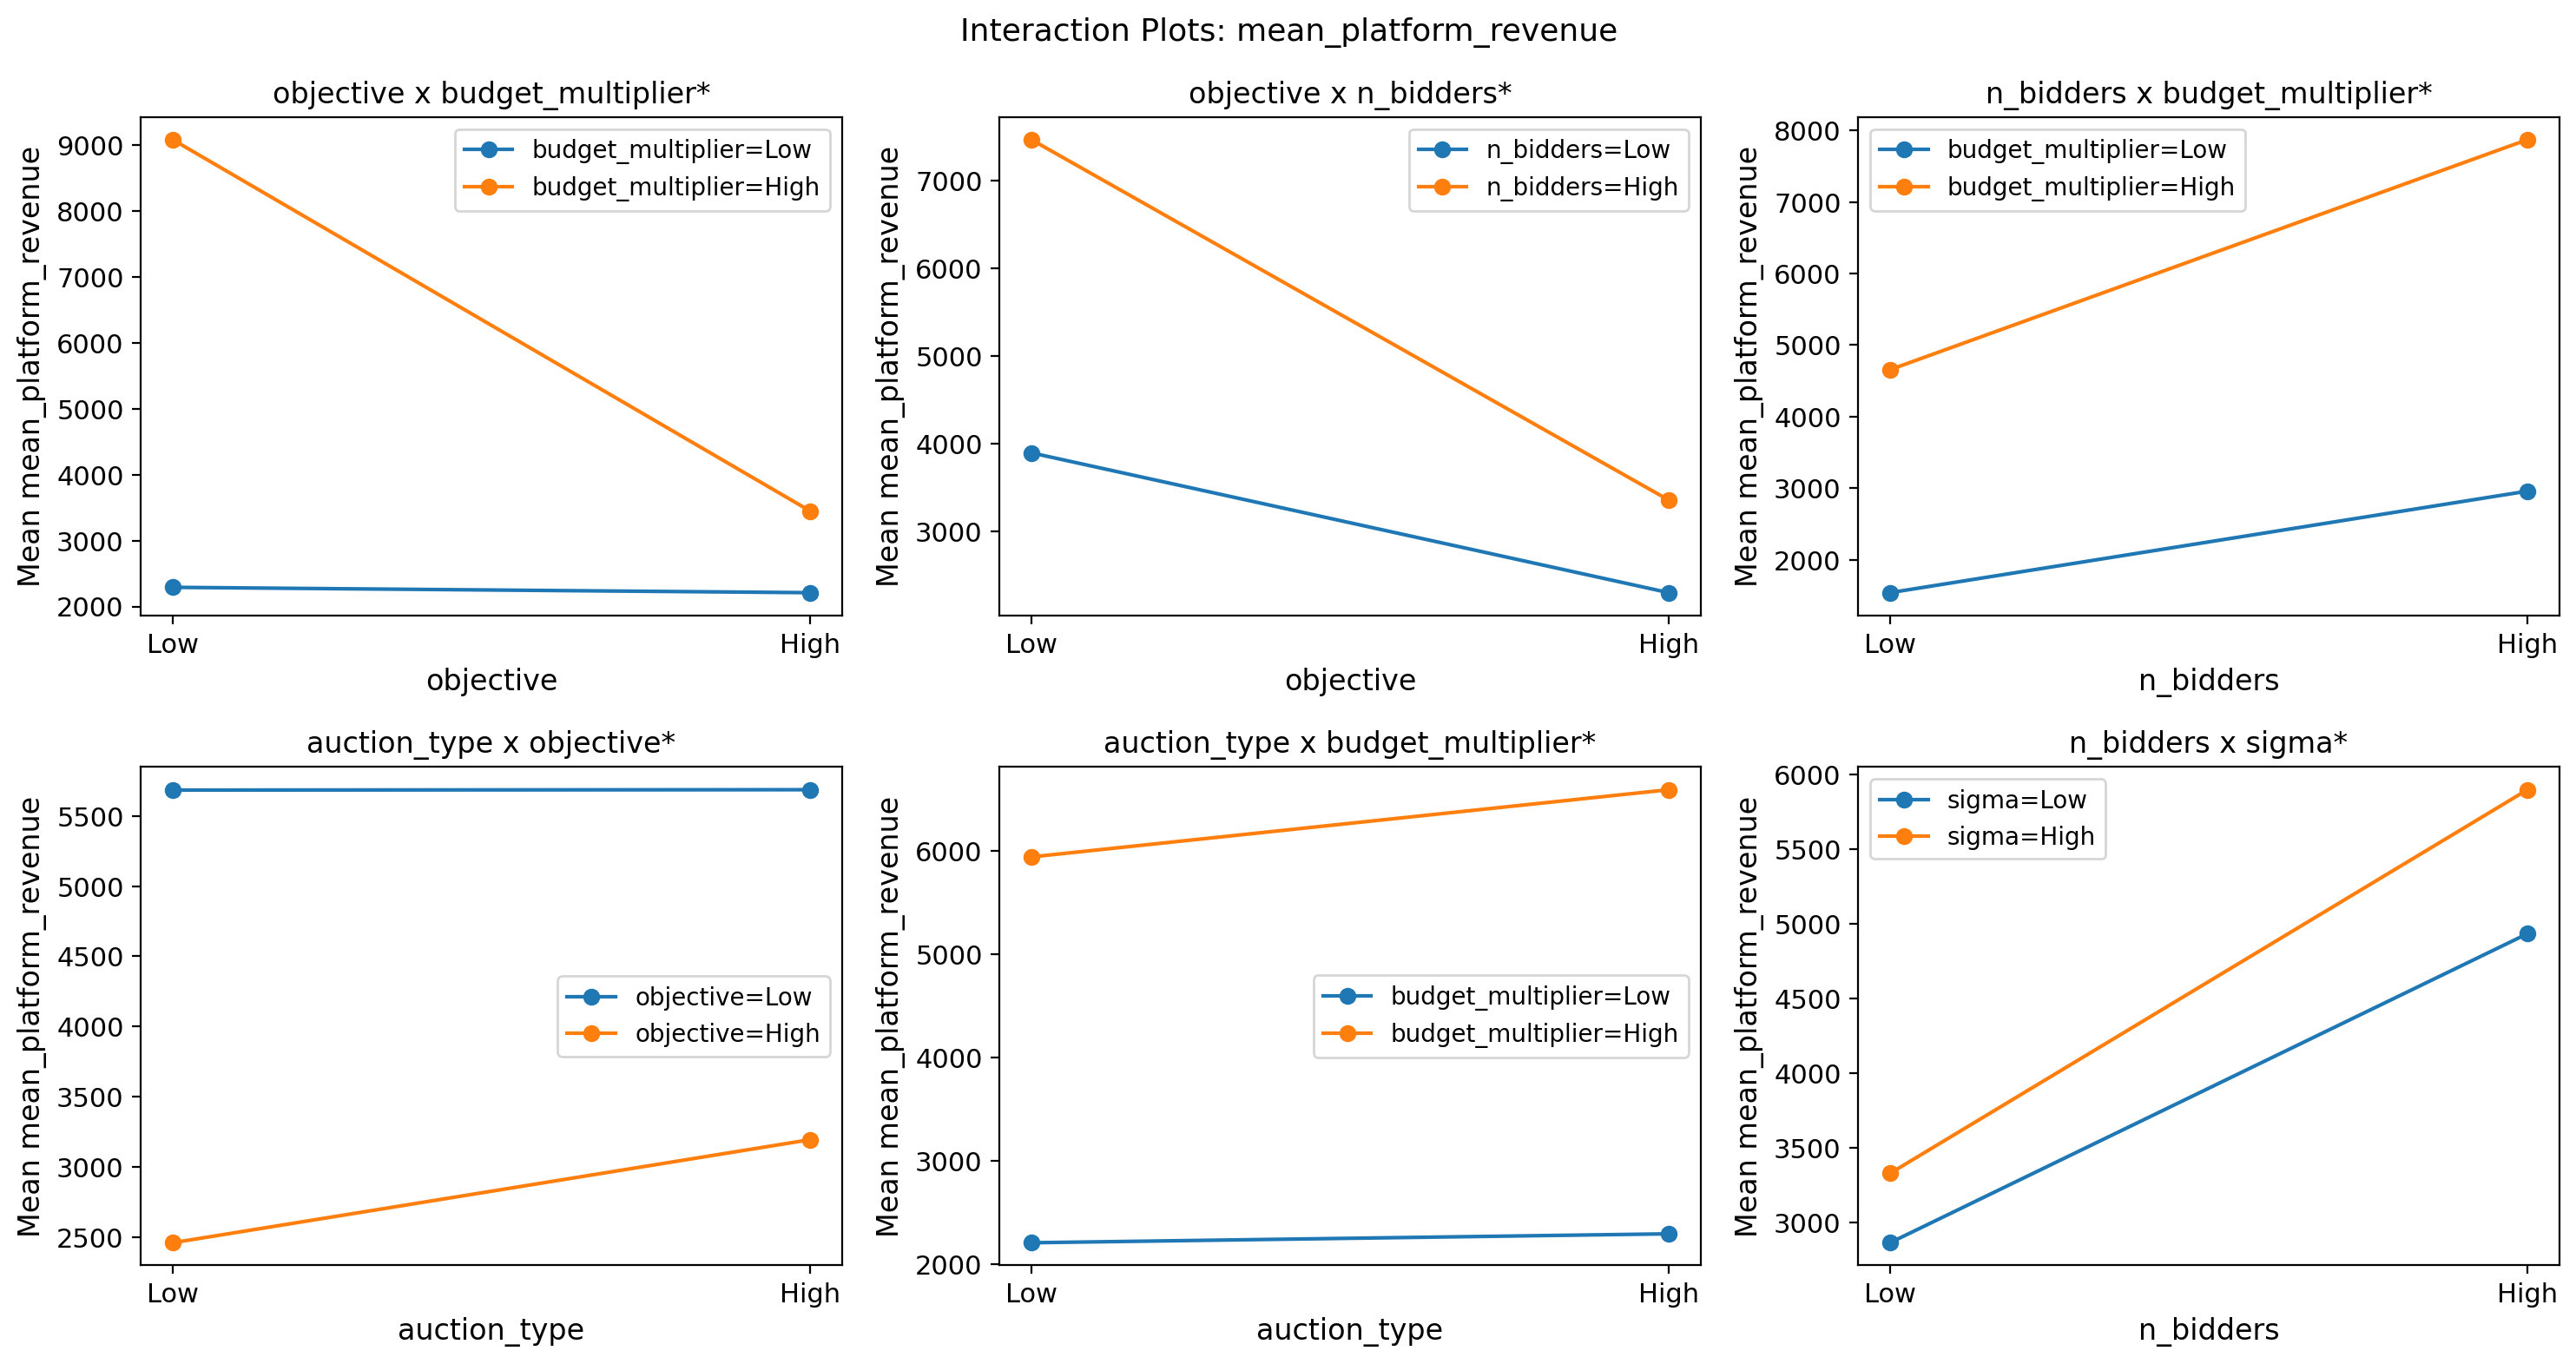
\includegraphics[width=0.7\textwidth]{figures/e3a_int_rev}
  \caption{Experiment~3a: Interaction plot for platform revenue.}
  \label{fig:e3a_int_rev}
\end{figure}

\subsubsection{Bidding Behaviour and Bid Suppression Indicators}

\begin{table}[H]
\centering
\caption{Experiment 3a: Significant effects for price volatility ($p < 0.05$), ranked by $|t|$.}
\label{tab:exp3a_ranked_vol}
\begin{tabular}{lrrl}
\toprule
\textbf{Effect} & \textbf{Coeff.} & \textbf{$|t|$} & \textbf{Direction} \\
\midrule
Budget multiplier & 1.2878 & 3.26 & + \\
Bidder objective & -1.1490 & 2.91 & $-$ \\
Bidder objective $\times$ Budget multiplier & -1.1266 & 2.85 & $-$ \\
Auction format & -0.8413 & 2.13 & $-$ \\
Auction format $\times$ Bidder objective & 0.7996 & 2.02 & + \\
Auction format $\times$ Value dispersion ($\sigma$) & -0.7853 & 1.99 & $-$ \\
\bottomrule
\end{tabular}
\end{table}


\begin{figure}[H]
  \centering
  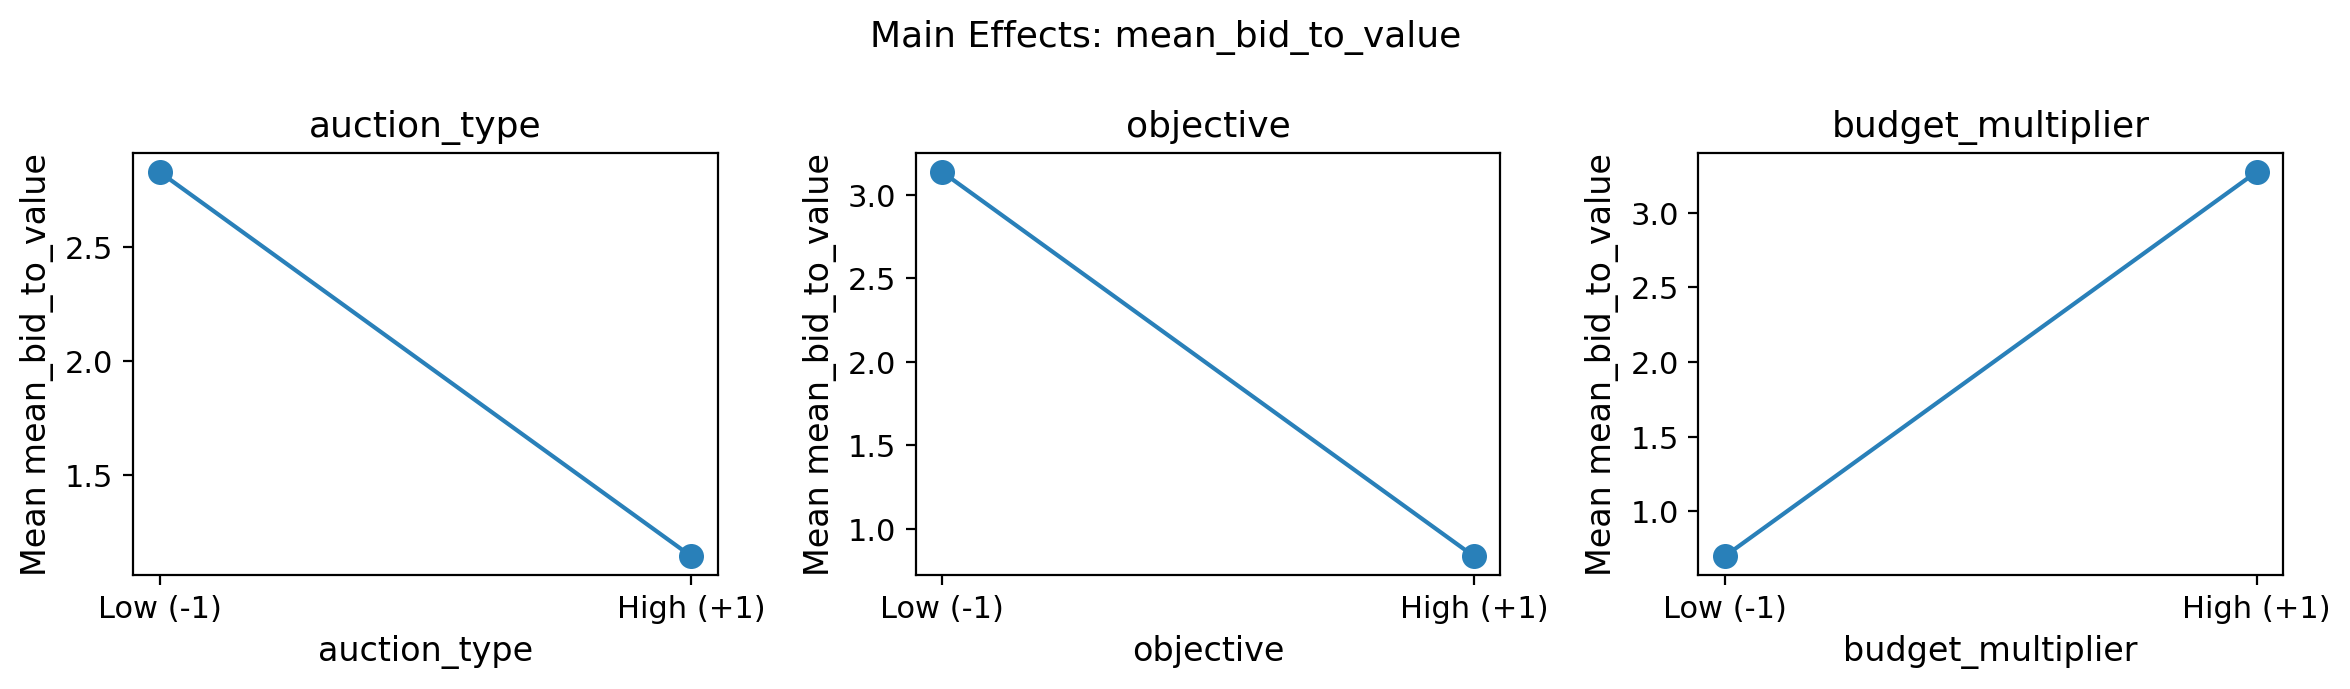
\includegraphics[width=0.7\textwidth]{figures/e3a_main_vol}
  \caption{Experiment~3a: Main effects plot for bid-to-value ratio.}
  \label{fig:e3a_main_vol}
\end{figure}

The factorial model explains \ExpThreeAWelfareRsqPct\% of the variance in liquid welfare but only \ExpThreeADriftRsqPct\% in cross-episode drift, reflecting substantial seed-level noise in the latter metric. Cross-episode drift, measured as the slope of the bid-to-value ratio across post-burn-in episodes, assesses the \citet{PaesLeme2024} prediction that bidders progressively suppress bids across campaign cycles. Although the factorial ANOVA for drift is statistically significant ($F$-test $p \ExpThreeADriftFPFmt$), the model explains only \ExpThreeADriftRsqPct\% of the variance ($R^2 = \ExpThreeADriftRsq$), and all cell-level drift estimates remain near zero.\footnote{The large sample size (\ExpThreeANobs{} runs) allows detection of statistically significant but economically negligible effects.} This near-zero drift falsifies the prediction of \citet{PaesLeme2024} that dual-based pacing produces progressive bid suppression.

\subsubsection{Learning Dynamics}

Warm-start benefits are dominated by bidder objective ($t = \ExpThreeAWarmObjT$). Under utility-maximizing objectives, warm-start produces measurable gains, while value-maximizing agents show negligible warm-start gains. Inter-episode volatility is similarly dominated by objective ($t = \ExpThreeAIEVolObjT$), with utility-maximizing agents exhibiting higher volatility. Model adequacy diagnostics (Appendix~\ref{sec:appendix_robustness}) confirm clean inference.\footnote{$R^2$ ranges from \ExpThreeARsqMin{} to \ExpThreeARsqMax, PRESS gaps are below \ExpThreeAPRESSGapMax, and \ExpThreeABHPct\% of significant effects survive Benjamini--Hochberg correction.}

\subsubsection{Summary}

The budget multiplier dominates revenue (\ExpThreeARevFactorOne{}, $|t| = \ExpThreeARevFactorTOne$), with bidder objective ranking second and their interaction third. The number of bidders ranks fourth ($|t| = \ExpThreeARevNbidAbsT$), and auction format is a comparatively minor factor ($|t| = \ExpThreeARevAuctionT$). Global sensitivity analysis confirms budget multiplier dominance across all response variables (Section~\ref{sec:sens_exp3a}).

\subsection{PI Controller Results (Experiment~3b)}
\label{sec:exp3b_results}

Experiment~3b uses the same $2^6$ factorial structure as Experiment~3a (Table~\ref{tab:exp3b_params}), replacing the bidder objective factor with aggressiveness. The 512 runs are analysed with the same factorial ANOVA engine.

\begin{figure}[H]
  \centering
  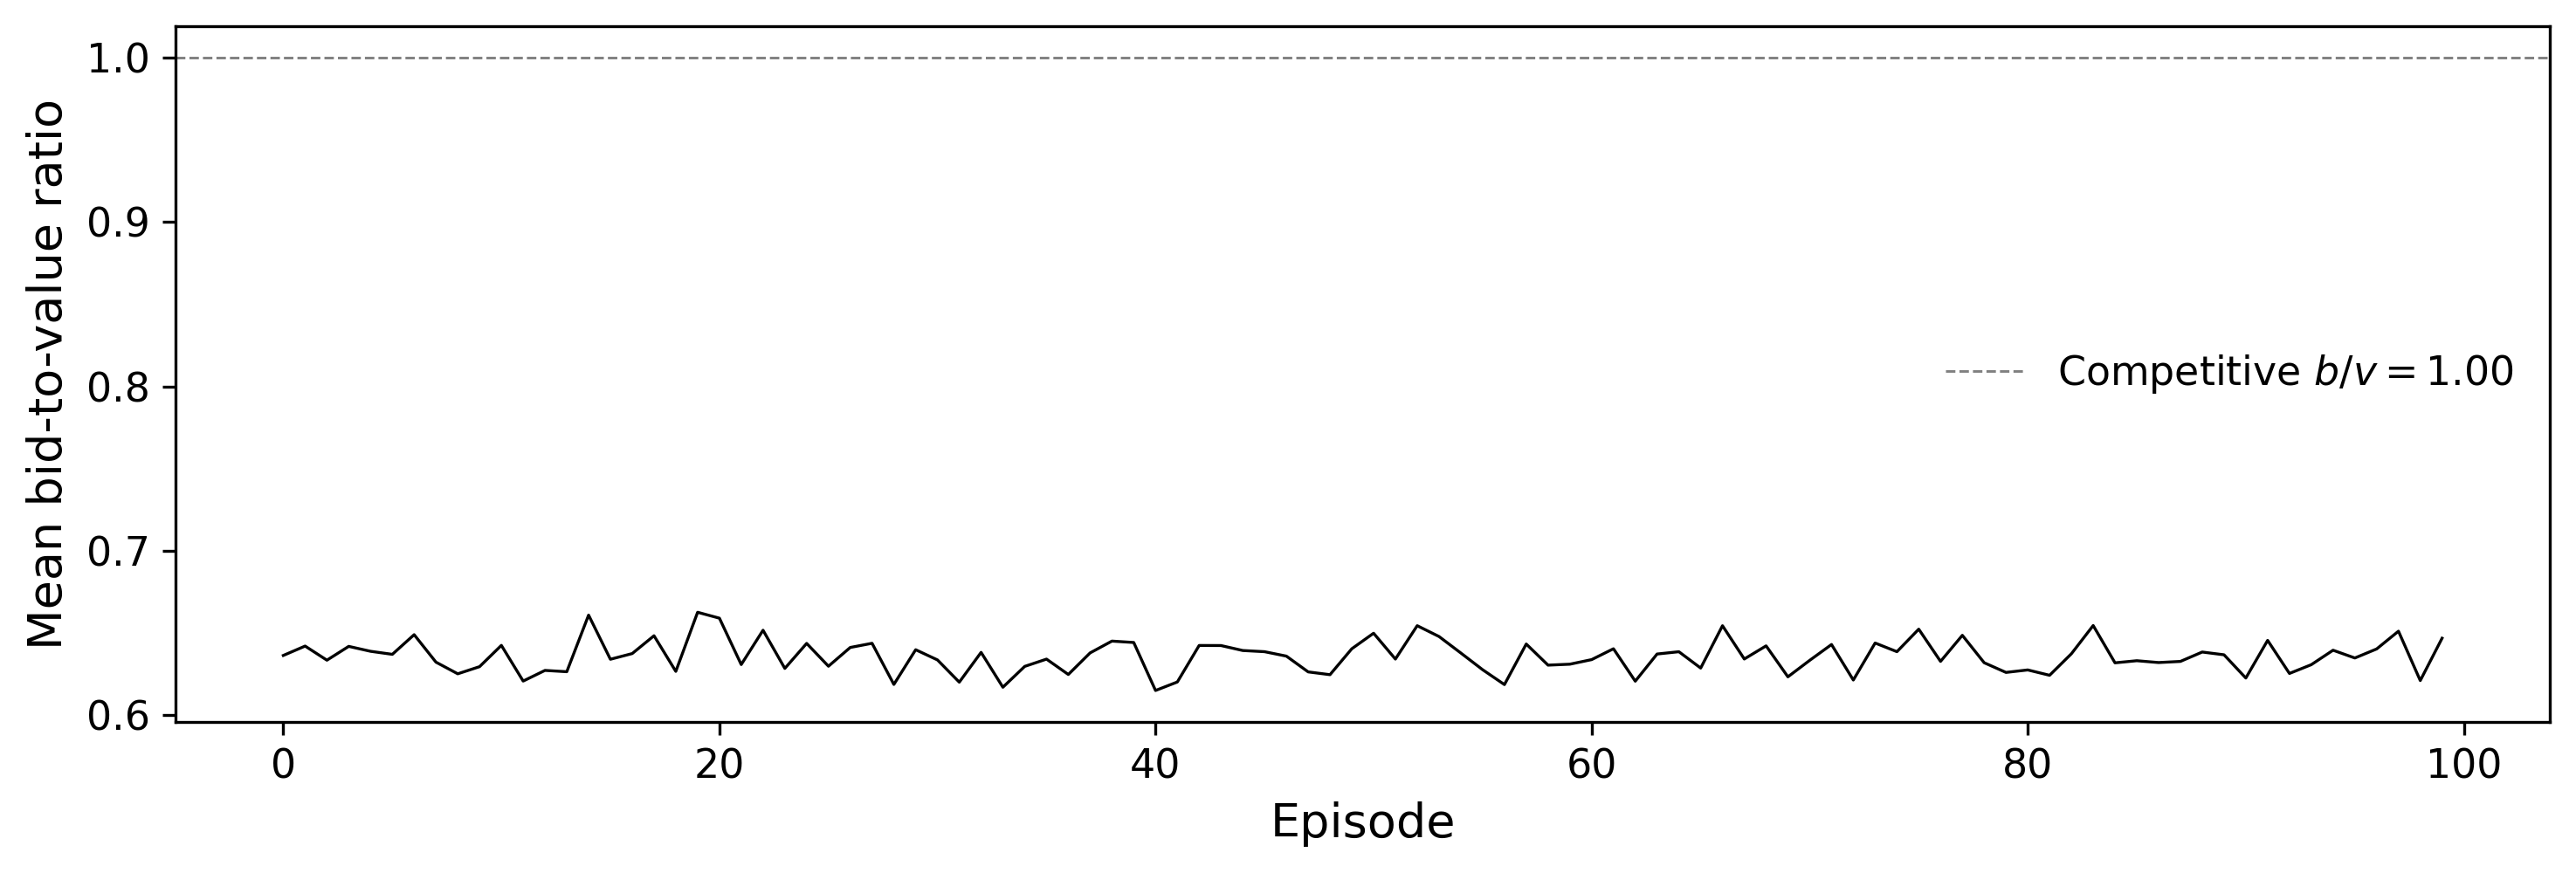
\includegraphics[width=\textwidth]{figures/e3b_trace}
  \caption{Representative learning trajectory for a single trial of Experiment~3b (first-price auction, default aggressiveness, 2~bidders, 100 episodes $\times$ 1{,}000 rounds). Mean bid-to-value ratio per episode with the competitive benchmark ($b/v = 1.0$).}
  \label{fig:e3b_trace}
\end{figure}

\subsubsection{Efficiency and Welfare}

The PI controller produces welfare outcomes that can be compared directly with the dual pacing results of Experiment~3a. Platform revenue and liquid welfare are computed identically, and the effective Price of Anarchy uses the same LP-based offline optimum as denominator. As in Experiment~3a, the budget multiplier dominates revenue (Table~\ref{tab:exp3b_ranked_rev}), with the effect amounting to \ExpThreeBRevTopPctEffect\% of the grand mean.

\begin{table}[H]
\centering
\caption{Experiment 3b: Significant effects for average revenue ($p < 0.05$), ranked by $|t|$.}
\label{tab:exp3b_ranked_rev}
\begin{tabular}{lrrl}
\toprule
\textbf{Effect} & \textbf{Coeff.} & \textbf{$|t|$} & \textbf{Direction} \\
\midrule
Budget multiplier & 1316.1821 & 31.68 & + \\
Number of bidders & 667.7779 & 16.07 & + \\
Auction format & 458.3301 & 11.03 & + \\
Auction format $\times$ Budget multiplier & 393.6340 & 9.47 & + \\
Value dispersion ($\sigma$) & 360.6121 & 8.68 & + \\
Auction format $\times$ Value dispersion ($\sigma$) & 233.6535 & 5.62 & + \\
Budget multiplier $\times$ Value dispersion ($\sigma$) & 175.0143 & 4.21 & + \\
Number of bidders $\times$ Value dispersion ($\sigma$) & 146.9008 & 3.54 & + \\
\bottomrule
\end{tabular}
\end{table}


\begin{figure}[H]
  \centering
  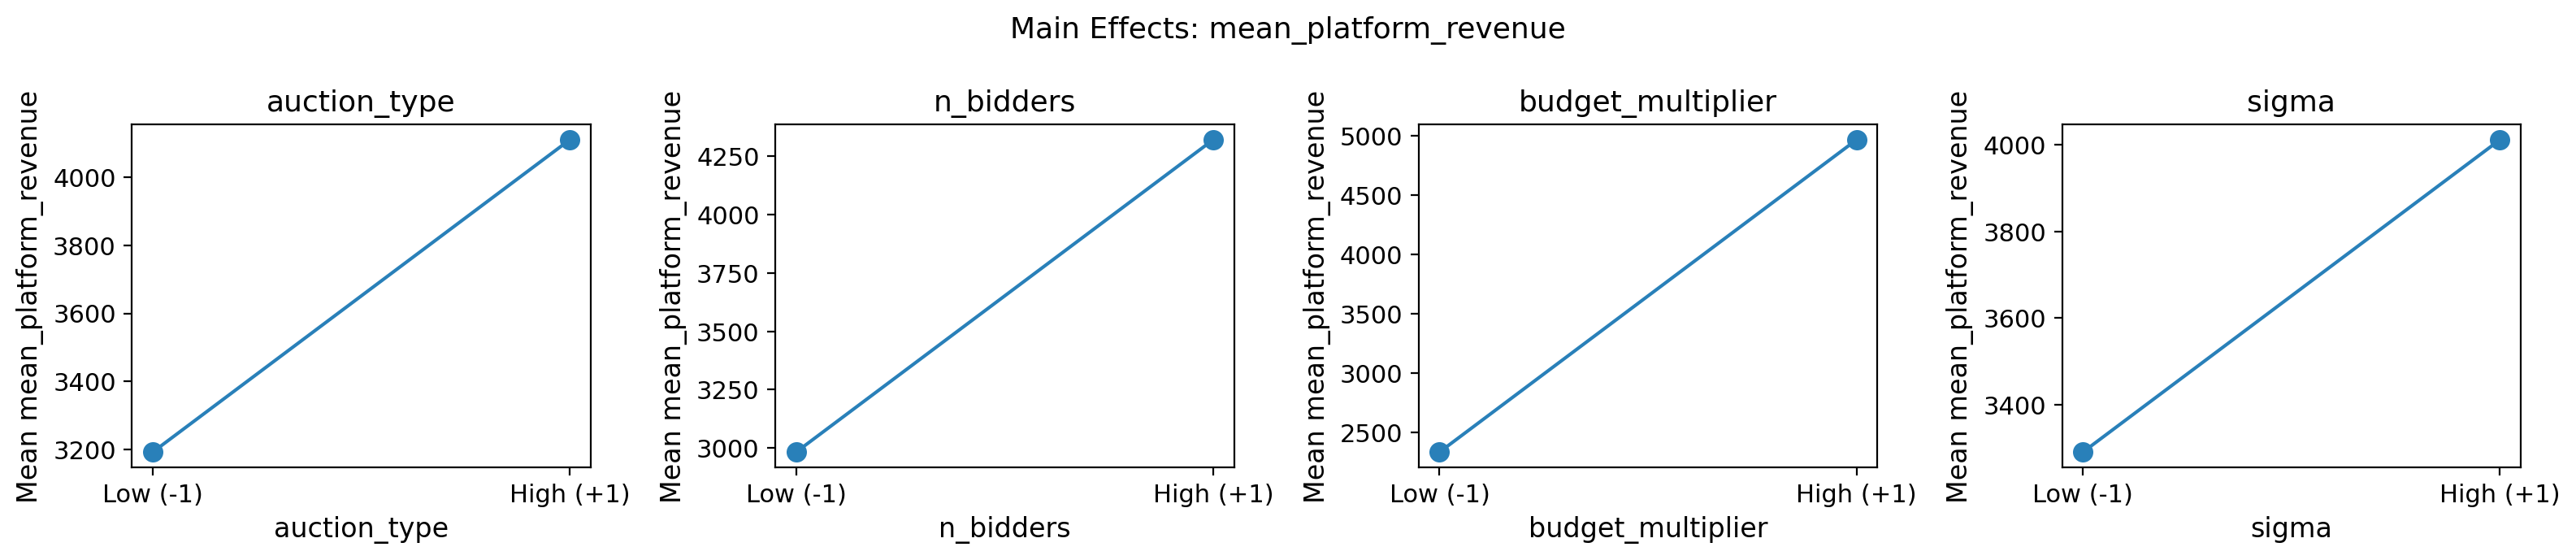
\includegraphics[width=0.7\textwidth]{figures/e3b_main_rev}
  \caption{Experiment~3b: Main effects plot for platform revenue.}
  \label{fig:e3b_main_rev}
\end{figure}

\begin{table}[H]
\centering
\caption[Experiment 3b: Significant effects for effective price of anarchy ($p < 0.05$), ranked by $|t|$]{\textbf{Experiment 3b: Significant effects for effective price of anarchy ($p < 0.05$), ranked by $|t|$.}}
\label{tab:exp3b_ranked_poa}
\begin{tabular}{lrrl}
\toprule
\textbf{Effect} & \textbf{Coeff.} & \textbf{$|t|$} & \textbf{Direction} \\
\midrule
Auction format & 0.0141 & 10.69 & + \\
Number of bidders $\times$ Budget multiplier & -0.0130 & 9.87 & $-$ \\
Auction format $\times$ Budget multiplier & 0.0073 & 5.56 & + \\
Value dispersion ($\sigma$) & -0.0064 & 4.84 & $-$ \\
Number of bidders & 0.0039 & 2.93 & + \\
Auction format $\times$ Reserve price & 0.0036 & 2.73 & + \\
Number of bidders $\times$ Reserve price & 0.0031 & 2.35 & + \\
Number of bidders $\times$ Value dispersion ($\sigma$) & -0.0029 & 2.21 & $-$ \\
Budget multiplier $\times$ Reserve price & -0.0029 & 2.18 & $-$ \\
Reserve price $\times$ Value dispersion ($\sigma$) & 0.0029 & 2.16 & + \\
\bottomrule
\end{tabular}
\end{table}


\begin{figure}[H]
  \centering
  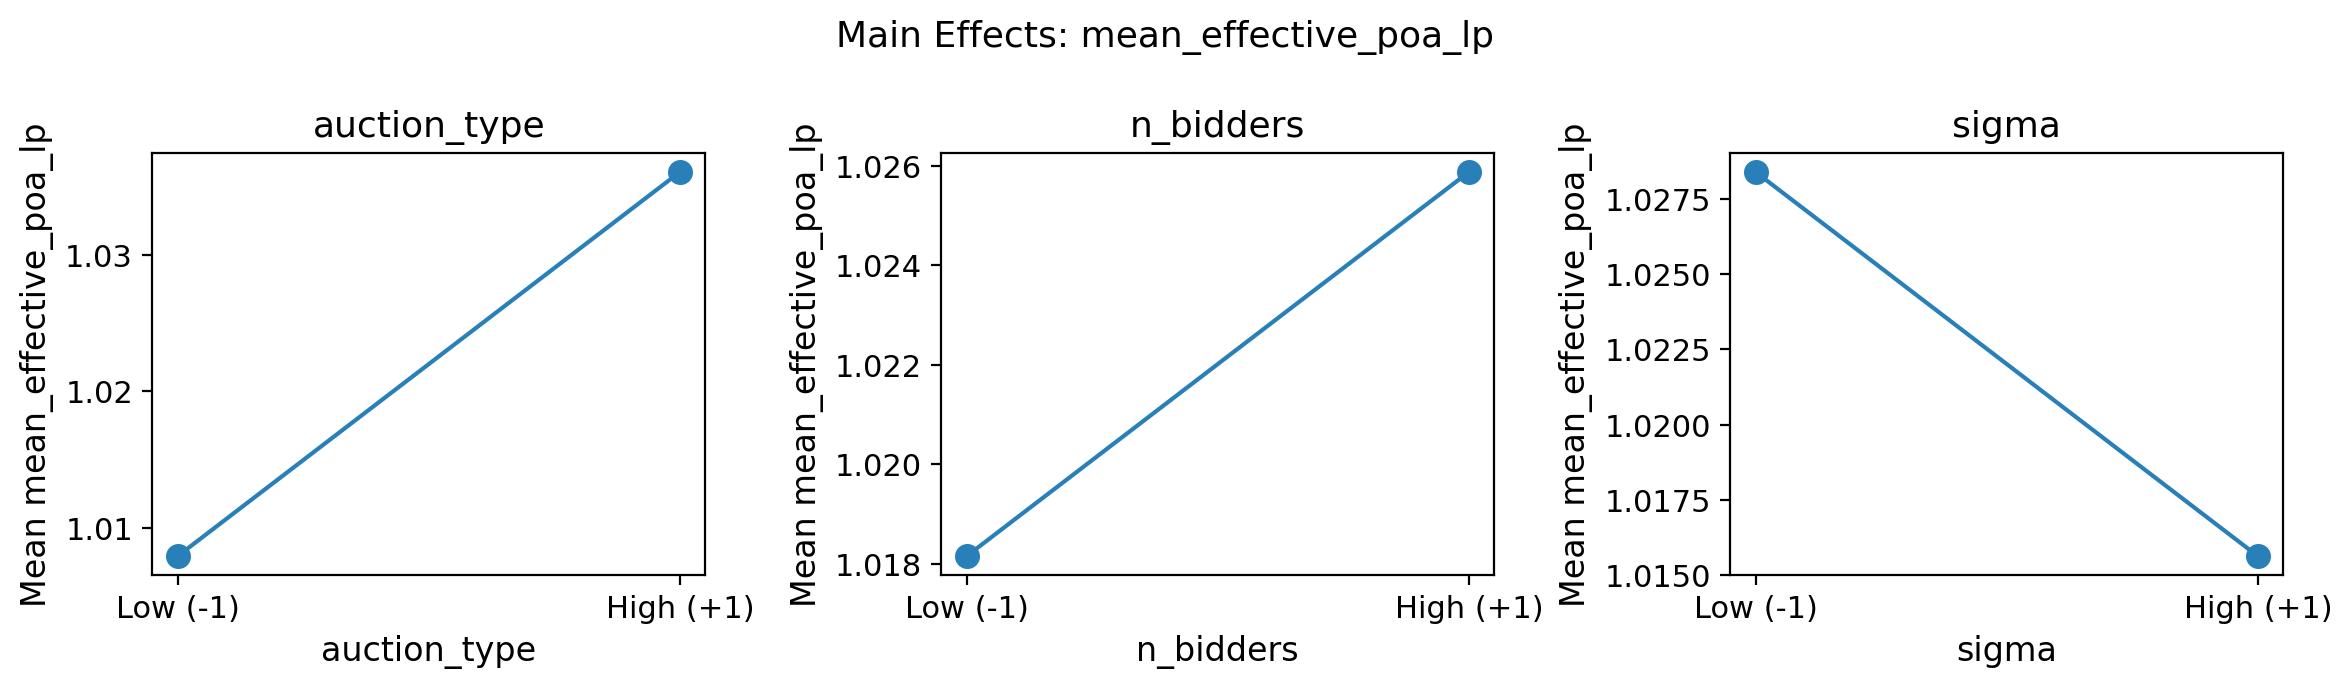
\includegraphics[width=0.7\textwidth]{figures/e3b_main_poa}
  \caption{Experiment~3b: Main effects plot for effective Price of Anarchy.}
  \label{fig:e3b_main_poa}
\end{figure}

For the effective Price of Anarchy, auction format is the dominant factor ($|t| = 10.7$), with first-price auctions producing higher PoA values. The number of bidders $\times$ budget multiplier interaction ranks second ($|t| = 9.9$). Thin markets with tight budgets generate the largest efficiency losses. Value dispersion reduces PoA ($|t| = 4.8$). As in Experiment~3a, all observed PoA values remain within the theoretical bound. Allocative efficiency follows a similar pattern. The budget multiplier dominates ($|t| = 44.7$), with loose budgets yielding near-efficient allocations.

\subsubsection{Revenue and Budget Dynamics}

The auction type $\times$ budget multiplier interaction is the strongest two-way effect on revenue ($|t| = 9.5$), indicating that the revenue advantage of first-price auctions is concentrated in loose-budget settings where agents can bid aggressively. Under tight budgets, both formats produce similar revenue as pacing constraints dominate. The auction type $\times$ value dispersion interaction ($|t| = 5.6$) shows that the first-price revenue advantage grows with value dispersion. The budget multiplier $\times$ value dispersion ($|t| = 4.2$) and number of bidders $\times$ value dispersion ($|t| = 3.5$) interactions round out the significant two-way effects. Figure~\ref{fig:e3b_int_rev} displays these interaction patterns.

\begin{figure}[H]
  \centering
  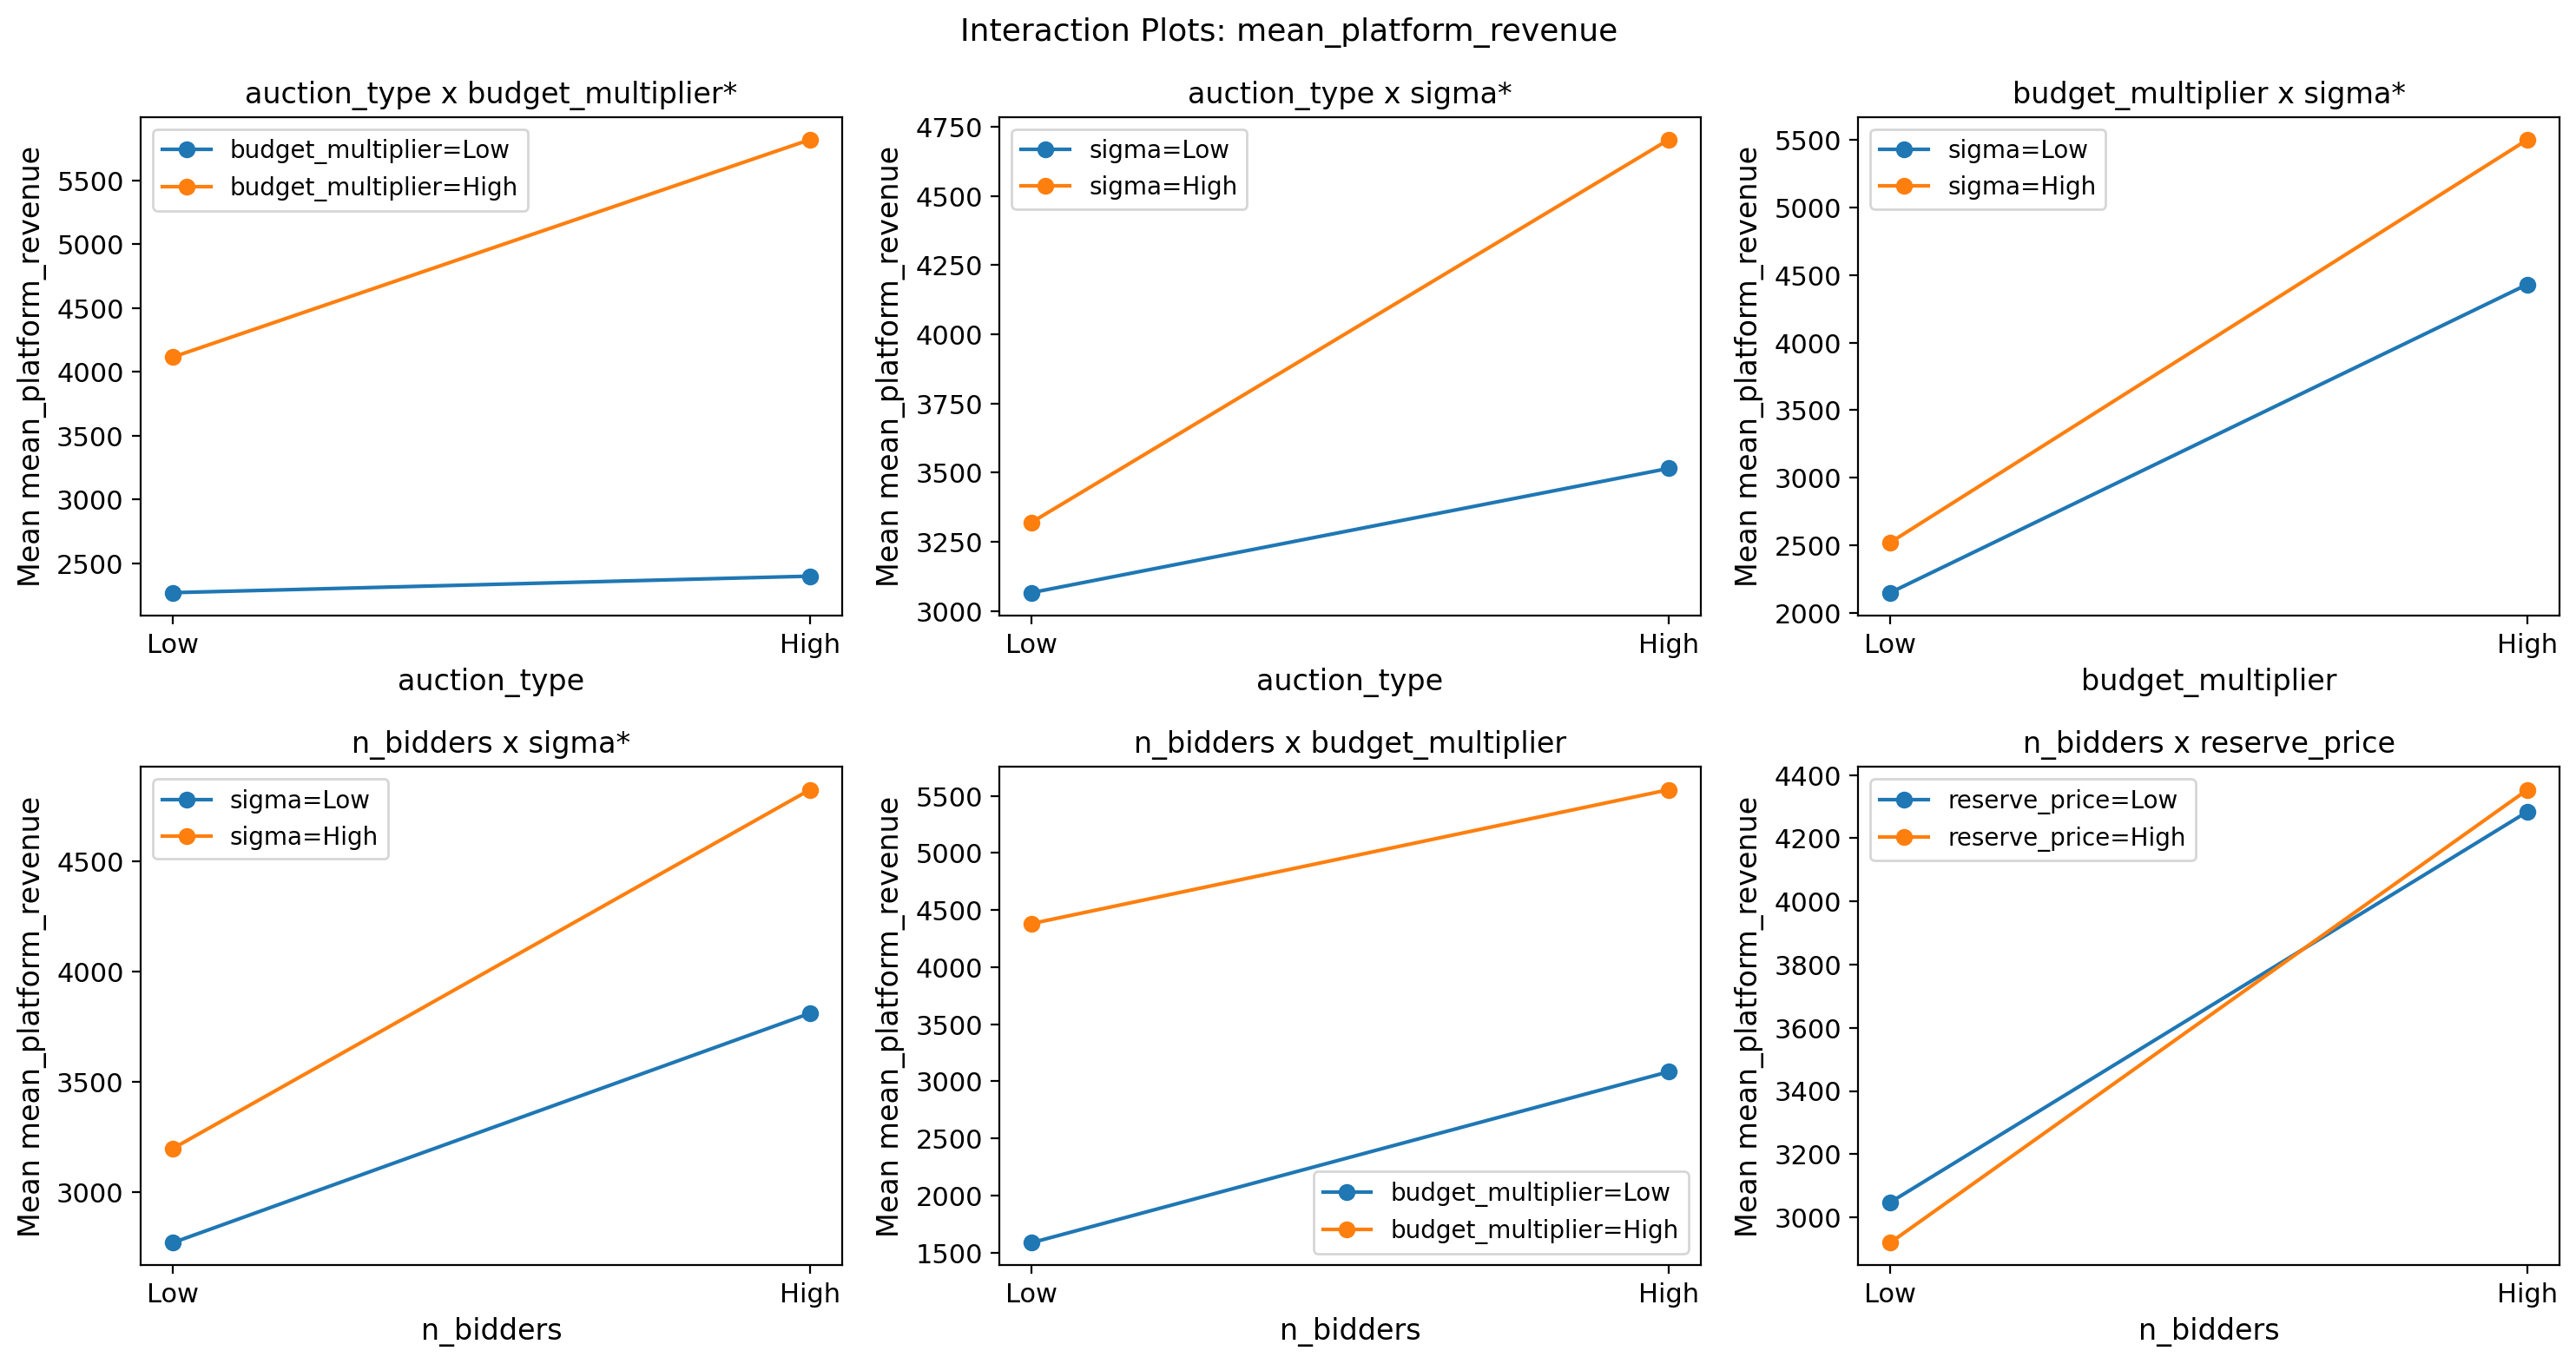
\includegraphics[width=0.7\textwidth]{figures/e3b_int_rev}
  \caption{Experiment~3b: Interaction plot for platform revenue.}
  \label{fig:e3b_int_rev}
\end{figure}

\subsubsection{Bidding Behaviour}

The bid-to-value ratio is well-explained by the factorial model ($R^2 = 0.89$). The budget multiplier is the dominant factor ($|t| = 54.4$). Loose budgets permit higher bids relative to value, while tight budgets force aggressive shading. Auction format ranks second ($|t| = 22.3$), with first-price auctions producing substantially lower bid-to-value ratios than second-price, consistent with the theoretical prediction that first-price bidders shade below value. The auction type $\times$ budget multiplier interaction ($|t| = 17.3$) indicates that bid shading under first-price rules is amplified when budgets are tight. The auction type $\times$ number of bidders interaction ($|t| = 5.8$) reflects that additional bidders narrow the bid-to-value gap between formats. Compared with the multiplicative pacing of Experiment~3a, the PI controller produces qualitatively similar bid-to-value patterns but with less extreme shading under tight budgets. Table~\ref{tab:exp3b_ranked_vol} and Figure~\ref{fig:e3b_main_vol} report the full effect hierarchy.

\begin{table}[H]
\centering
\caption{Experiment 3b: Significant effects for price volatility ($p < 0.05$), ranked by $|t|$.}
\label{tab:exp3b_ranked_vol}
\begin{tabular}{lrrl}
\toprule
\textbf{Effect} & \textbf{Coeff.} & \textbf{$|t|$} & \textbf{Direction} \\
\midrule
Budget multiplier & 0.3873 & 54.37 & + \\
Auction format & -0.1585 & 22.25 & $-$ \\
Auction format $\times$ Budget multiplier & 0.1233 & 17.31 & + \\
Auction format $\times$ Number of bidders & 0.0410 & 5.76 & + \\
\bottomrule
\end{tabular}
\end{table}


\begin{figure}[H]
  \centering
  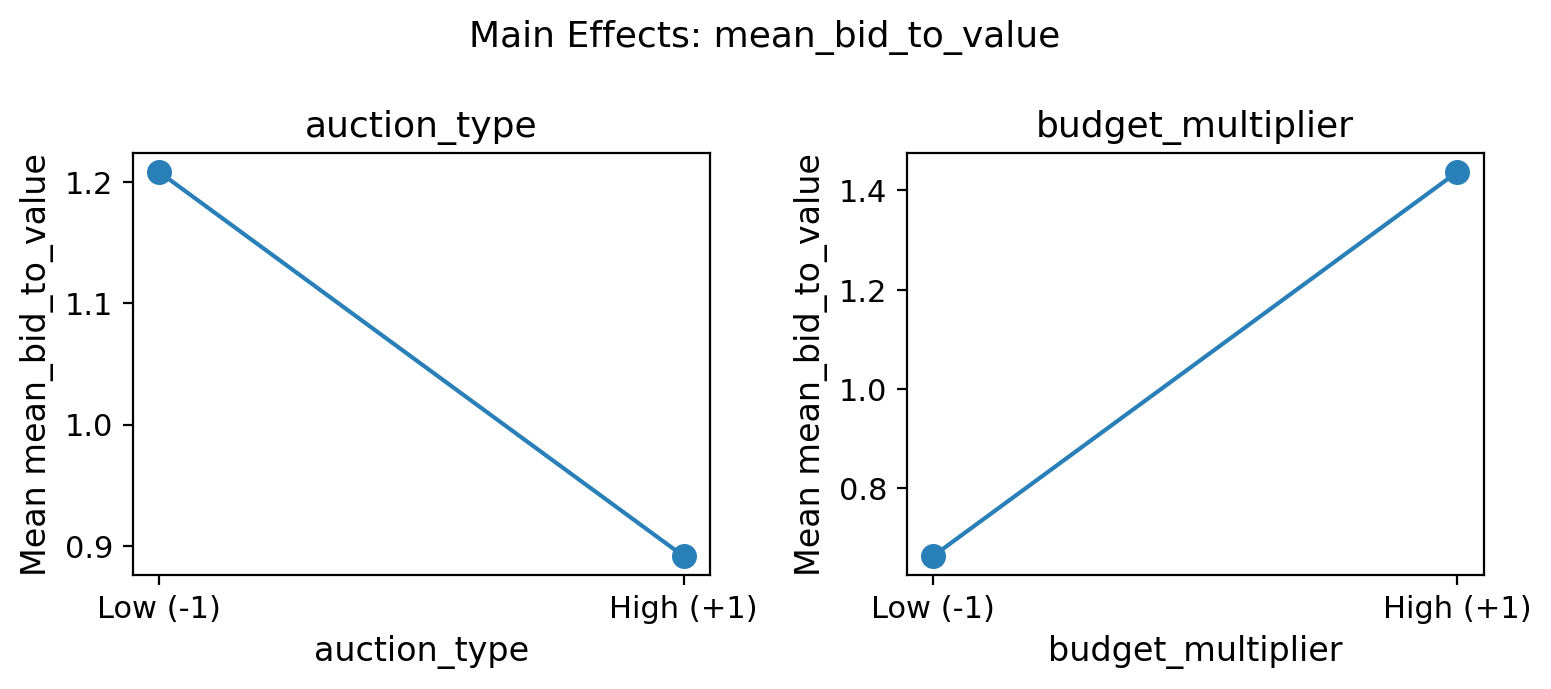
\includegraphics[width=0.7\textwidth]{figures/e3b_main_vol}
  \caption{Experiment~3b: Main effects plot for bid-to-value ratio.}
  \label{fig:e3b_main_vol}
\end{figure}

\subsection{Sensitivity Analysis}
\label{sec:sens_pacing}

\subsubsection{Experiment~3a: Dual Pacing Autobidders}
\label{sec:sens_exp3a}

Budget multiplier is the dominant factor for seven of fourteen responses, including revenue ($S_T = 0.54$), liquid welfare ($S_T = 0.52$), and pacing stability ($S_T = 0.43$). The bidder objective dominates budget utilisation ($S_T = 0.66$), allocative efficiency ($S_T = 0.48$), and effective price of anarchy ($S_T = 0.35$). Auction format and reserve price are negligible across primary responses ($S_T < 0.04$). Cross-method concordance is strong ($\rho = 0.72$). Detailed Sobol' indices appear in Appendix~\ref{sec:appendix_sensitivity_tables} (Tables~\ref{tab:sens_exp3a_primary}--\ref{tab:sens_exp3a_secondary}).

\subsubsection{Experiment~3b: PI Controller Pacing}
\label{sec:sens_exp3b}

Budget multiplier again dominates the majority of responses, including revenue ($S_T = 0.53$) and budget utilisation ($S_T = 0.70$). A notable difference from Experiment~3a emerges for the price of anarchy and inter-episode volatility, where auction format becomes the most important factor ($S_T = 0.19$ and $0.33$ respectively), whereas it was negligible under dual pacing. Aggressiveness is negligible across all responses ($S_T < 0.04$). Cross-method concordance is strong ($\rho = 0.77$). Detailed Sobol' indices appear in Appendix~\ref{sec:appendix_sensitivity_tables} (Tables~\ref{tab:sens_exp3b_primary}--\ref{tab:sens_exp3b_secondary}).

\subsubsection{Cross-Method Concordance}
\label{sec:sens_concordance}

Table~\ref{tab:sens_concordance} summarises the agreement among the seven sensitivity methods across all experiments. The mean pairwise Spearman rank correlation provides a scalar measure of whether different methods agree on which factors matter most. Concordance is highest for Experiment~1a ($\rho = 0.87$) and Experiment~3b ($\rho = 0.77$), both of which have clear dominant factors and large sample sizes. Concordance is lowest for Experiment~2b ($\rho = 0.04$), where many factors have similar total-order indices and the methods disagree on their relative ranking. In all experiments, the identity of the top one or two factors is consistent across methods even when the full ranking shows disagreement; the low concordance values primarily reflect instability in the ordering of minor factors.

\begin{table}[H]
\centering
\caption{Cross-method concordance: mean pairwise Spearman $\rho$ across seven sensitivity methods, averaged over all response variables within each experiment.}
\label{tab:sens_concordance}
\small
\begin{tabular}{lcc}
\toprule
Experiment & Mean Spearman $\rho$ & Number of responses \\
\midrule
1a: Q-Learning (constant)       & 0.87 & 5 \\
1b: Q-Learning (affiliated)     & 0.33 & 8 \\
2a: LinUCB                     & 0.33 & 5 \\
2b: Thompson Sampling          & 0.04 & 5 \\
3a: Dual Pacing                & 0.72 & 16 \\
3b: PI Pacing                  & 0.77 & 16 \\
\bottomrule
\end{tabular}
\end{table}

\subsection{Summary}

The comparison between multiplicative dual pacing and PI control isolates the role of the control mechanism from the budget constraint itself. In both experiments, the budget multiplier is the dominant revenue driver ($|t| = \ExpThreeARevFactorTOne$ in Experiment~3a; $|t| = \ExpThreeBRevFactorTOne$ in Experiment~3b), confirming that budget tightness, not the pacing algorithm, is the primary determinant of revenue outcomes. The number of bidders ranks among the top factors in both cases ($|t| = \ExpThreeARevNbidAbsT$ in 3a; $|t| = 16.1$ in 3b), while auction format plays a stronger role under PI control ($|t| = 11.0$) than under dual pacing ($|t| = \ExpThreeARevAuctionT$). PoA values remain within the theoretical bound in both experiments (Section~\ref{sec:exp3a_results}). The two pacing mechanisms produce different bid-to-value ratio levels, but the factor hierarchy is consistent across both approaches, indicating that the structural features of the budget-constrained environment dominate the choice of control algorithm. This consistency further distinguishes constraint-driven from learning-driven bid suppression. In Experiments~1a--2b, switching algorithms changed the direction of the auction-format effect, whereas here, switching the pacing mechanism leaves the format effect unchanged. Global sensitivity analysis independently confirms these rankings (Sections~\ref{sec:sens_exp3a}--\ref{sec:sens_exp3b}). Cross-method concordance is strong in both cases ($\rho = 0.72$ in 3a, $\rho = 0.77$ in 3b), indicating robust agreement across all seven sensitivity methods (Section~\ref{sec:sens_concordance}).

\label{sec:sens_synthesis}

Table~\ref{tab:sens_dominant} summarises the dominant factor for each response variable that is comparable across multiple experiments. The entries report the factor with the highest total-order index and its $S_T$ value.

\begin{table}[H]
\centering
\caption{Dominant factor (highest $S_T$) for comparable responses across experiments. Factor abbreviations: N = number of bidders, R = reserve price, A = auction format, B = budget multiplier, O = bidder objective.}
\label{tab:sens_dominant}
\small
\setlength{\tabcolsep}{4pt}
\begin{tabular}{l cccccc}
\toprule
Response & Exp~1a & Exp~1b & Exp~2a & Exp~2b & Exp~3a & Exp~3b \\
\midrule
Revenue        & N (0.24) & N (0.22) & N (0.55) & N (0.31) & B (0.54) & B (0.53) \\
Conv.\ time    & N (0.11) & A (0.11) & N (0.21) & N (0.16) & -- & -- \\
No-sale rate   & R (0.27) & -- & R (0.45) & N (0.41) & B (0.40) & B (0.33) \\
Volatility     & N (0.17) & N (0.17) & A (0.24) & N (0.37) & -- & -- \\
Winner entropy & N (0.31) & N (0.16) & N (0.75) & N (0.32) & N (0.63) & N (0.58) \\
\midrule
Eff.\ PoA      & -- & -- & -- & -- & O (0.35) & A (0.19) \\
Liq.\ welfare  & -- & -- & -- & -- & B (0.52) & B (0.50) \\
Budget util.   & -- & -- & -- & -- & O (0.66) & B (0.70) \\
Alloc.\ eff.   & -- & -- & -- & -- & O (0.48) & B (0.74) \\
\bottomrule
\end{tabular}
\end{table}

Market structure is the primary determinant of algorithmic auction outcomes across all six experiments. In the four learning experiments (1a, 1b, 2a, 2b), the number of bidders is the dominant factor for revenue in every case, achieving total-order indices from 0.22 to 0.55 (Table~\ref{tab:sens_dominant}). It also dominates winner entropy in all six experiments ($S_T = 0.16$--$0.75$), reflecting the mechanical relationship between market size and competitive balance. In the two autobidding experiments (3a, 3b), budget multiplier replaces number of bidders as the dominant revenue factor ($S_T = 0.53$--$0.54$) and drives most welfare and efficiency metrics. This transition is consistent with the theoretical distinction between the two experimental families: in learning experiments the number of competitors determines equilibrium revenue, while in autobidding the budget constraint is the binding force that shapes market outcomes.

Reserve price and auction format occupy distinct niches in the factor importance hierarchy. Reserve price is the dominant factor for no-sale rate in Experiments~1a and~2a ($S_T = 0.27$ and $0.45$), confirming its direct role as a bid-acceptance threshold. In Experiment~2b, reserve price ranks second to the number of bidders for no-sale rate ($S_T = 0.41$ vs $0.41$), essentially tied. Auction format is rarely the top-ranked factor; across 51 well-fitted response variables, it is dominant in only five cases.\footnote{Well-fitted responses are those with $R^2 > 0.15$, excluding three Experiment~3a responses and two Experiment~3b responses where the model explains negligible variance.} Its strongest contributions are to winner's curse frequency in Experiment~1b ($S_T = 0.36$), inter-episode volatility in Experiment~3b ($S_T = 0.33$), price volatility in Experiment~2a ($S_T = 0.24$), effective price of anarchy in Experiment~3b ($S_T = 0.19$), and convergence time in Experiment~1b ($S_T = 0.11$). The choice between first-price and second-price formats thus matters most for stability and strategic behaviour rather than for aggregate revenue.

Algorithmic tuning parameters are consistently negligible across all four algorithm families tested. In Experiment~1a, learning rate ($\alpha$), decay type, and initialisation each have $S_T < 0.03$ across all five responses. In Experiments~2a and 3b, regularisation ($\lambda$), memory decay, and exploration intensity fall below $S_T = 0.04$ for both revenue and no-sale rate. In Experiment~3b, the aggressiveness parameter has $S_T < 0.04$ for every response. This pattern suggests that market outcomes are robust to moderate variation in algorithmic hyperparameters, and that the market environment matters far more than the algorithm's internal configuration.

Interaction effects are pervasive across all experiments. The gap between total-order and first-order indices ($S_T - S_1$) frequently exceeds 0.10, indicating that a factor's influence on the response depends substantially on the levels of other factors. This pattern is most pronounced for the no-sale rate in Experiment~2b, where three factors each have $S_T > 0.33$ despite $S_1 < 0.20$. Even dominant factors operate partly through interactions: the number of bidders in Experiment~2b has $S_1 = 0.18$ but $S_T = 0.31$ for revenue, and budget multiplier in Experiment~3a has $S_1 = 0.35$ but $S_T = 0.54$. The residual fraction (variance not explained by any first- or second-order term) ranges from 0.04 (Experiment~3a budget utilisation) to 0.97 (Experiment~3b warm-start benefit), reflecting both replication noise and higher-order interactions beyond the two-way terms in the model. These interaction effects mean that isolated factor-by-factor analysis can substantially understate a factor's true importance, reinforcing the value of total-order indices over first-order indices alone.
